\subsection{Определение интегрируемой функции и интеграла Римана. Необходимое условие интегрируемости}

\subsubsection*{1. Определения}

Рассмотрим функцию $f(x)$, заданную на отрезке $[a, b]$. Для определения интеграла Римана вводится понятие разбиения отрезка.

\begin{definition}[Разбиение]
\textbf{Разбиением} $P$ отрезка $[a, b]$ называется конечный набор точек $x_0, x_1, \dots, x_n$, таких что:
\[ a = x_0 < x_1 < x_2 < \dots < x_n = b \]
Точки $x_j$ называются точками разбиения, а отрезки $[x_{j-1}, x_j]$ — элементарными отрезками разбиения. Длина $j$-го отрезка обозначается $\Delta x_j = x_j - x_{j-1}$.
\end{definition}

\begin{definition}[Параметры разбиения]
\textbf{Диаметром (мелкостью)} разбиения $P$ называется величина $\lambda(P)$, равная максимальной из длин элементарных отрезков:
\[ \lambda(P) = \max_{1 \le j \le n} \Delta x_j \]
\textbf{Набором отмеченных точек} $\xi$ называется совокупность точек $\xi_j$, выбранных произвольным образом на каждом элементарном отрезке: $\xi_j \in [x_{j-1}, x_j]$.
\end{definition}

\begin{definition}[Интегральная сумма Римана]
\textbf{Интегральной суммой Римана} функции $f(x)$ для данного разбиения $P$ и набора отмеченных точек $\xi$ называется величина:
\[ \sigma(f, P, \xi) = \sum_{j=1}^n f(\xi_j) \Delta x_j \]
Геометрически, если $f(x) \ge 0$, эта сумма представляет собой площадь ступенчатой фигуры, составленной из прямоугольников с основаниями $\Delta x_j$ и высотами $f(\xi_j)$.
\end{definition}

\begin{definition}[Интеграл Римана]
Число $I$ называется \textbf{пределом интегральных сумм} при $\lambda(P) \to 0$, если:
\[ \forall \eps > 0 \quad \exists \delta > 0 : \forall P, \lambda(P) < \delta \implies \forall \xi \quad |\sigma(f, P, \xi) - I| < \eps \]
Если такой предел существует и конечен, то функция $f(x)$ называется \textbf{интегрируемой по Риману} на отрезке $[a, b]$ ($f \in R([a, b])$), а сам предел называется \textbf{определенным интегралом Римана} и обозначается:
\[ I = \int\limits_a^b f(x) dx \]
\end{definition}

\subsubsection*{2. Необходимое условие интегрируемости}

Лектор отмечает, что интегрируемость накладывает серьезные ограничения на поведение функции, в частности, на её ограниченность.

\begin{theorem}[Необходимое условие интегрируемости]
Если функция $f(x)$ интегрируема по Риману на отрезке $[a, b]$, то она \textbf{ограничена} на этом отрезке.
\end{theorem}

\begin{tcolorbox}[title=Доказательство, breakable]
Докажем от противного. Пусть функция $f(x)$ интегрируема на $[a, b]$, но не ограничена на нем. 

Согласно критерию Коши для интегральных сумм, для любого $\eps > 0$ (возьмем $\eps = 1$) существует $\delta > 0$, такое что для любого разбиения $P$ с $\lambda(P) < \delta$ и любых двух наборов отмеченных точек $\xi'$ и $\xi''$ выполняется:
\[ |\sigma(f, P, \xi') - \sigma(f, P, \xi'')| < 1 \]

Зафиксируем произвольное разбиение $P$ с диаметром $\lambda(P) < \delta$. Так как функция $f(x)$ не ограничена на всем отрезке $[a, b]$, она должна быть не ограничена хотя бы на одном из элементарных отрезков этого разбиения. Пусть это отрезок $[x_{k-1}, x_k]$.

Выберем два набора отмеченных точек $\xi'$ и $\xi''$, которые совпадают во всех индексах $j \neq k$:
\[ \xi'_j = \xi''_j \text{ при } j \neq k \]
Тогда разность интегральных сумм примет вид:
\[ |\sigma(f, P, \xi') - \sigma(f, P, \xi'')| = |f(\xi'_k) \Delta x_k - f(\xi''_k) \Delta x_k| = |f(\xi'_k) - f(\xi''_k)| \Delta x_k \]

Поскольку функция $f(x)$ не ограничена на $[x_{k-1}, x_k]$, мы можем зафиксировать $\xi''_k$ и выбирать $\xi'_k$ так, чтобы значение $|f(\xi'_k)|$ было сколь угодно великим. Следовательно, величину $|f(\xi'_k) - f(\xi''_k)| \Delta x_k$ можно сделать больше любого наперед заданного числа (в том числе больше 1).

Это противоречит критерию Коши. Следовательно, наше предположение было неверным, и интегрируемая функция обязана быть ограниченной.
\end{tcolorbox}

\subsubsection*{3. Геометрический смысл}
Интеграл Римана $\int_a^b f(x) dx$ для неотрицательной функции численно равен площади криволинейной трапеции — фигуры, ограниченной графиком функции $y=f(x)$, осью $Ox$ и вертикальными прямыми $x=a$ и $x=b$. Если функция принимает значения разных знаков, интеграл равен разности площадей частей фигуры, лежащих выше и ниже оси абсцисс.

%\begin{center}
%\includegraphics[width=0.6\textwidth]{riemann_sum_geometry.png}
% На рисунке должен быть изображен график функции f(x), разбиение отрезка [a, b] 
% на интервалы и прямоугольники, высоты которых определяются точками xi_j.
%\end{center}

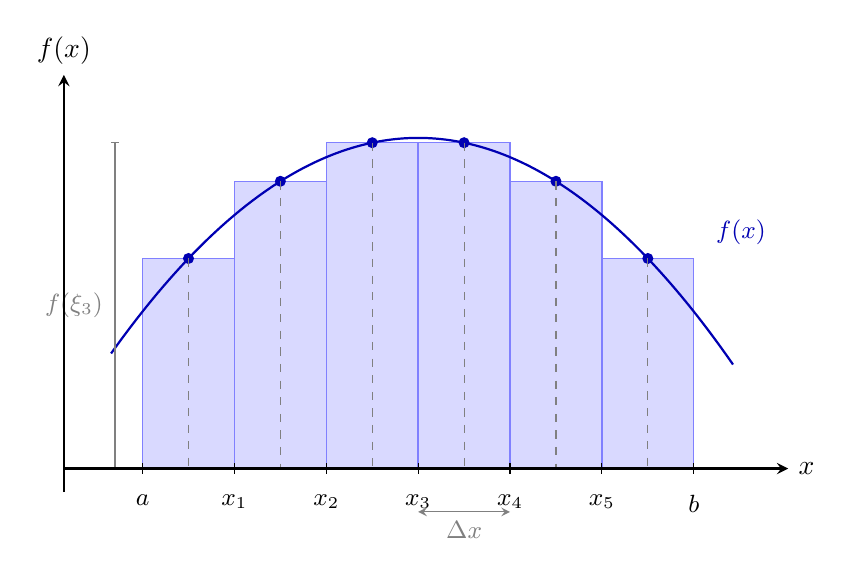
\begin{tikzpicture}[scale=1.0, >=stealth]
 
% --- Параметры ---
\def\xa{1.0}   % a
\def\xb{8.0}   % b
\def\yn{0.0}   % уровень оси x
 
% --- Функция f(x): гладкий горб ---
% f(x) = -0.18*(x-4.5)^2 + 4.2
\pgfmathdeclarefunction{myfunc}{1}{%
  \pgfmathparse{-0.18*(#1-4.5)^2 + 4.2}%
}
 
% --- Разбиение: 6 подотрезков ---
% x0=1, x1=2.167, x2=3.333, x3=4.5, x4=5.667, x5=6.833, x6=8
% xi_j — середины подотрезков
\def\dx{1.1667}
 
% Заливка прямоугольников (снизу вверх, до f(xi_j))
\foreach \j/\xi in {1/1.583, 2/2.750, 3/3.917, 4/5.083, 5/6.250, 6/7.417} {
  \pgfmathsetmacro{\xleft}{\xa + (\j-1)*\dx}
  \pgfmathsetmacro{\xright}{\xa + \j*\dx}
  \pgfmathsetmacro{\ht}{-0.18*(\xi-4.5)^2 + 4.2}
  \fill[blue!15, draw=blue!50, line width=0.5pt]
    (\xleft, \yn) rectangle (\xright, \ht);
}
 
% --- Кривая f(x) поверх прямоугольников ---
\draw[blue!70!black, thick, domain=0.6:8.5, samples=120]
  plot (\x, {-0.18*(\x-4.5)^2 + 4.2});
 
% --- Точки xi_j на кривой ---
\foreach \xi in {1.583, 2.750, 3.917, 5.083, 6.250, 7.417} {
  \pgfmathsetmacro{\ht}{-0.18*(\xi-4.5)^2 + 4.2}
  \fill[blue!70!black] (\xi, \ht) circle (2pt);
  % Пунктирная вертикаль от xi_j до оси
  \draw[gray, dashed, thin] (\xi, \ht) -- (\xi, \yn);
}
 
% --- Подписи xi_j на оси x ---
%\foreach \j/\xi/\lab in {
%    1/1.583/{$\xi_1$},
%    2/2.750/{$\xi_2$},
%    3/3.917/{$\xi_3$},
%    4/5.083/{$\xi_4$},
%    5/6.250/{$\xi_5$},
%    6/7.417/{$\xi_6$}} {
%  \node[below, blue!70!black, font=\small] at (\xi, \yn) {\lab};
%}
 
% --- Деления x_j на оси x ---
\foreach \j/\lab in {
    0/{$a$},
    1/{$x_1$},
    2/{$x_2$},
    3/{$x_3$},
    4/{$x_4$},
    5/{$x_5$},
    6/{$b$}} {
  \pgfmathsetmacro{\xpos}{\xa + \j*\dx}
  \draw (\xpos, \yn+0.07) -- (\xpos, \yn-0.07);
  \node[below=6pt, font=\small] at (\xpos, \yn) {\lab};
}
 
% --- Скобка f(xi_3) для третьего прямоугольника ---
\pgfmathsetmacro{\hthree}{-0.18*(3.917-4.5)^2 + 4.2}
\draw[gray, thin]
  (0.65, \yn) -- (0.65, \hthree);
\draw[gray, thin] (0.60, \yn) -- (0.70, \yn);
\draw[gray, thin] (0.60, \hthree) -- (0.70, \hthree);
\node[left, font=\small, gray] at (0.62, \hthree/2) {$f(\xi_3)$};
 
% --- Стрелка Delta x ---
\pgfmathsetmacro{\xleftfour}{\xa + 3*\dx}
\pgfmathsetmacro{\xrightfour}{\xa + 4*\dx}
\draw[<->, gray, thin] (\xleftfour, -0.55) -- (\xrightfour, -0.55)
  node[midway, below, font=\small, gray] {$\Delta x$};
 
% --- Оси координат ---
\draw[->, thick] (0, 0) -- (9.2, 0) node[right] {$x$};
\draw[->, thick] (0, -0.3) -- (0, 5.0) node[above] {$f(x)$};
 
% --- Подпись кривой ---
\node[blue!70!black, font=\itshape\small] at (8.6, 3.0) {$f(x)$};
 
% --- Формула ---
 
\end{tikzpicture}

$\displaystyle S = \sum_{j=1}^{n} f(\xi_j)\,\Delta x_j
  \;\longrightarrow\;
  \int_a^b f(x)\,dx
  \quad \text{при } \|\Delta\| \to 0$
